\section{Liner Shipping Operations}
\subsection{Cargo and vessel}
Unsurprisingly, the cargo for container vessels consist for the most part of containers in standardized sizes. The most common sizes are 20' or 40' long containers with a width of 8' and a height of 8'6''. Containers with a length of 45', and containers with a height of 9'8'' also exists but are less common. Of these commonly sized container, some -- known as \emph{reefers} -- are used to transport goods that requires refrigeration, and these containers needs to be powered under transport.  The weight of the containers varies, but the cargo/containers are not uncommonly divided into weight classes denoted by an average weigth (for example, 5t, 13t, etc.).

The stowage area on a container vessel is divided into a grid of \emph{cells}, each of which can hold two 20' containers or one 40' (or 45') (see Figure~\ref{fig:vesselA}). Some of the cells have power plugs, which means that reefer containers can be stowed herein. 
Stacks of containers are arranged longitudinal in \emph{bays} consisting of stacks \emph{on deck} and \emph{below deck} (see Figure~\ref{fig:vesselA}), and each stack rests on sockets with a maximum weight limit. 
\emph{Hatch covers} separate the cargo on deck from the cargo below deck, and each hatch cover spans a number of bays in one direction and a number of stacks in the other direction (see Figure~\ref{fig:overstowA}).
For modelling purposes, the vessel is divided into \emph{sections} longitudinally consisting of zero or more bays together with the space in between (see Figure~\ref{fig:vesselA}). 

To help achieve stability of the vessel, large water ballast tanks are placed on the vessel (see Figure~\ref{fig:vesselA}). Other tanks containing e.g. bunker fuel and fresh water is also placed along the vessel.

\begin{figure}[pos=htbp]
	\centering
		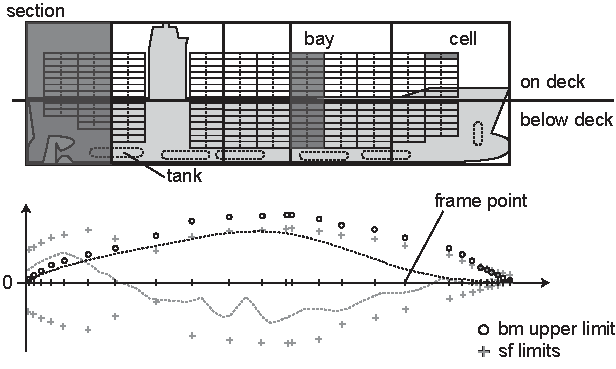
\includegraphics{figures/vessel1.pdf} 
	\caption{Vessel structure and limits for shear force (sf) and bending moment (bm) at frame points. The actual values of these forces are shown too \red{(but should they?)}.}
	\label{fig:vesselA}
\end{figure}

\subsection{Stowage considerations}
Stowing a container vessel is not as easy as it may sound initially, since many details regarding the cargo must be taken into consideration.
Below we will elaborate on some of these issues. The reader is referred to the recent book \cite{JPAV18} for more details.

%Capacity. 
Like with seats on an air-plane, there is a nominal upper bound on how many 20' and 40' containers, the stacks can hold. Likewise, only some of the cells have power plugs for reefer containers, limiting the number of these containers that can be stowed. These capacities are measured in \emph{twenty-foot equivalent units} (TEUs). 

%Hydrostatics. 
Though the number of containers is within the nominal capacities and the weight limits are also complied with, this does not guarantee the  seaworthiness of the vessel. When sailing, stress forces arise along the longitudinal axis of the vessel. These forces arise as a result of gravitation from the weight of cargo, tanks, and the vessel itself acting downwards and buoyancy from the water acting upwards. The resulting hydrostatic forces (stress forces, bending moments and transversal moments) must be within limits in order for the ship not to be impaired too much. These limits are given at certain positions along the vessel, known as \emph{frame points}. 

%GM and lashing (transversal stability).  
The metacentric height (GM) of a vessel is a measure relating to the transversal stability of the vessel against overturning. It is the distance between the center of gravity (G) of the vessel and the \emph{metacenter} M. M is found on a heeling vessel as the intersection of the centerline of the (transversally symmetric) vessel and a vertical line through the center of buoyancy (B) (see Figure~\ref{fig:GMA}). The higher GM is, the higher the transversal stability is (\cite{JPAV18}), and to avoid capsizing, it is therefore relevant to have this measure within given limits. 
On the other hand, GM affects other factors of stowing the vessel, e.g. lashing, where {higher} values of GM causes high acceleration forces \red{when the vessel is "correcting"}, meaning that less cargo can be securely stowed with lashing equipment. 

\begin{figure}
	\centering
	\begin{minipage}{.5\textwidth}
  		\centering
  		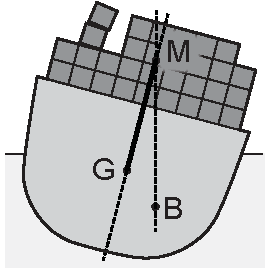
\includegraphics{figures/GM.pdf}
  		\caption{The metacentric heigh (GM) of a heeling vessel.}
  		\label{fig:GMA}
	\end{minipage}%
	\begin{minipage}{.5\textwidth}
  		\centering
  		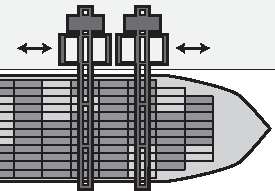
\includegraphics{figures/cranes.pdf}
  		\caption{Two cranes working on a part of a vessel.}
  		\label{fig:cranes}
	\end{minipage}
\end{figure}

The circumstances at the ports where the cargo has to be loaded and discharged also has to be considered. 
The main concern here is the crane movements required to stow the vessel as planned/wanted, since crane movements both take time and have a cost associated. 
A crane operates at a bay at a time, and it takes time for it to move from one bay to another. Cranes cannot pass each other (i.e., they have to stay in the same order) and due to their size/width, they cannot work at adjacent bays (see Figure~\ref{fig:cranes}). The cranes operating on the vessel operate at the same time, but all crane movements have to be done within the time that the vessel is allotted at the port (or alternatively: the cost measured in time has to be considered, if time is unlimited). Thus, the crane taking the longest time should also be finished within the time frame.

Discharging any container cannot always be done with just one simple discharge move. When a container is discharged, there can be no containers on top of it, and if it is below deck, there can be no containers on the hatch cover above it (see Figure~\ref{fig:overstowA}). Thus, if a container below deck is topped by containers in this was \emph{that needs to stay on board}, then these containers have to be first unloaded and then loaded again. This is very expensive and time consuming, which should be reflected in the model. 

\begin{figure}
	\centering
		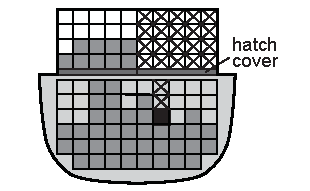
\includegraphics{figures/overstow.pdf}
	\caption{To move the black container, the crossed out cells must be empty (hatch covers exaggerated).}
	\label{fig:overstowA}
\end{figure}

When stowing, empty containers should be regarded as any other cargo, in the sense that they take up capacity and contribute to stress forces etc., and the moves that they give rise to should also be considered.    